\chapter{Technical details}\label{ch:technical}
This chapter will revolve around the technical aspect of implementing the system used for the experiment. The first section will talk about the software, before the second section talk about the different hardware accessories that were designed and used.


\section{Application implementation}
With the framework decided we were able to start creating our system. 
Throughout the process of creating the application we focused on refactoring options, configurations and settings in each component into their own components. These options/settings would at a later stage be gathered together and some were exposed through the user interface in order to make it possible to change the behaviour of the application at runtime. The process of always putting all the configuration and options in the same place made it possible for the system to be extremely extendable and modifiable. 

\bigskip\noindent
The main part of the application were developed using javascript, HTML and CSS, as these are the primary technologies used when creating application with the Apache Cordova framework. We will therefore keep the focus on these technologies, even though some minor adjustments where done in the native android controller to enable a higher debugging level than the bluetooth plugin had originaly.

\bigskip\noindent
Figure~\ref{fig:class} shows a simple "`class diagram"' of the application as it was when the project was coming to an end. Note that the term class diagram is not completely accurate as javascript is not a object oriented programming language in the same sense as Java, but utilizes prototypical inheritance to reuse common code components. The code for this application however isn't powered by a complicated class hierarchy and thus using the "`class diagram"' is sufficient to show how different components of the application interact.

\image{images/class.png}{\linewidth}{"`Class diagram"' of the javascript application}{fig:class}

\bigskip\noindent
The class diagram in figure~\ref{fig:class} shows a total of eighteen different javascript files, most of whom contain a single javascript "`class"', though some do contain several classes, but these classes are at an abstraction level below what should be exposed by the parent class. 

\bigskip\noindent
The main responsibilities of each class is shown in table~\ref{table:technical}.

\smalltable{Class descriptions}{table:technical}{
	\begin{longtable}{ll}
		Class name & Descriptions\\\hline \endfirsthead
		Class name & Descriptions\\\hline \endhead
		\\\hline \endfoot
		\\\hline \endlastfoot
		\textbf{main.js} & \wrap{Provides the entrypoint for the application. This file does not contain any classes, but have the responsibility of starting the application up, initializing all the other classes and handling the majority of events delegation.}{}\\
		\textbf{Program.js} & \wrap{Provides the Program class, which is responsibel for the extraction and validation of the program from either the graphical interface or the textual interface.}{}\\
		\textbf{RunnableProgram.js} & \wrap{Is a wrapper around the Program model responsible for preparsing of the program in the cases where pure javascript have been written.}{}\\
		\textbf{Options.js} & \wrap{A centralized locations for all application settings. Provides persistent storage of settings, and a simple user interface creator for generating the options menu.}{}\\
		\textbf{Keyboard.js} & \wrap{A simple class responsible for creating and handling a on-screen-keyboard.}{}\\
		\textbf{Codeblock.js} & \wrap{Another model class which stores the information of a single command. Marshalling and unmarshalling from and to the graphical and textual interface are handled by this model, but usually called at the \textit{Program} level.}{}\\
		\textbf{CodeblockManager.js} & \wrap{Responsible for inserting available codeblocks into the header of the application, and helping with the marshalling of textual blocks.}{}\\
		\textbf{CodeblockDefinitions.js} & \wrap{Provides the definition of all available codeblocks in the system, and how the different codeblocks should be translated into javascript. }{}\\
		\textbf{Device.js} & \wrap{An abstraction layer for removing any device dependencies and allowing the application to be tested on a computer by mocking different device dependent components.}{}\\
		\textbf{jsEngine.js} & \wrap{A generator class responsible for converting the Program or pure javascript into actual commands which can be sent to the robot.}{}\\
		\textbf{SimulatorFactory.js} & \wrap{The class responsible for keeping track of which of the four simulator types to use. This class listens to changes in bluetooth connectivity in order to allways provide the correct simulator.}{}\\
		\textbf{*Simulator.js} & \wrap{Refers to all the differet simulators. These classes takes a RunnableProgram as the argument, and spins up the correct simulator. In cases where a robot is connected they also have the responsibility of sending the commands and keeping in sync with the robot.}{}\\
		\textbf{*Bluetooth.js} & \wrap{Refers to both bluetooth classes. Based on a debugging flag in the application one of these classes will be started. MockBluetooth will keep the same to the same interface as Bluetooth, but will use stubbing methods in order to provide a testing surface for the bluetooth functionality.}{}\\
		\textbf{ConnectionUI.js} & \wrap{The bluetooth connection user interface is dynamically injected if a bluetooth enabled device is detected by the application. The UI is maintained by this class.}{}\\
	\end{longtable}
}

\bigskip\noindent
To see the resulting software please see appendix~\ref{appendix:appIntro}, which gives an introduction to the application.

\section{Hardware accessories}
After the mainpart of the application was created we still had a lot of work ahead of us before we had a working prototype. In order to make the robot ready for the experiment we still missed the contraption which would handle the drawing with the physical robot, and the bluetooth modules that were to mounted on top of the robot. 

\subsection{Chassis modifications}
The problem we initially underestimated was how we should make the physical robot draw on paper. While a front or back mounted pen would be an easy solution this would not create the angles properly, and thus was not a real viable options. The clearence below the robot was to small for anything to fit underneath it, and the battery was placed in such a way that nothing could fit between the wheels of the robot (see figure~\ref{fig:robotUnder}). In order to fix this problem we designed a batteryholder which could be mounted on top of the robot (see figure~\ref{fig:batteryHolder}), but due to techinical problems witht the 3D printes we were not able to test this design. And we had to resort to an alternative solution using velcro to position the battery at the back of the robot and duct tape to add a counterweight at the front of the robot to provide stability (see figures in~\ref{fig:robot}). 

\bigskip\noindent
While this solved the problem of making room beneath the robot we still had multiple issues with getting the robot to draw properly. These issues were mainly due to inaccuracies in the 3D-printing environment meaning the the spring used to push the drawing tip into the paper would get snagged inside its container (figures~\ref{fig:pencilHolder} and~\ref{fig:pencilHolderReal}).


\begin{figure}[H]
	\centering
	\subfloat[Battery holder\label{fig:batteryHolder}]{
		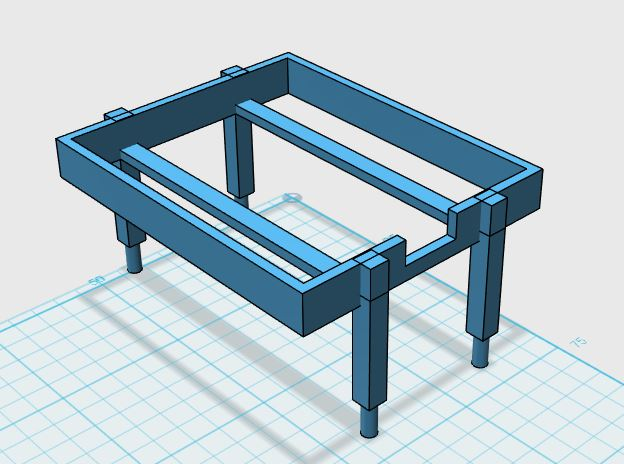
\includegraphics[width=0.4\linewidth]{images/BatteryHolder.JPG}
	}
	\subfloat[Pencil holder\label{fig:pencilHolder}]{
		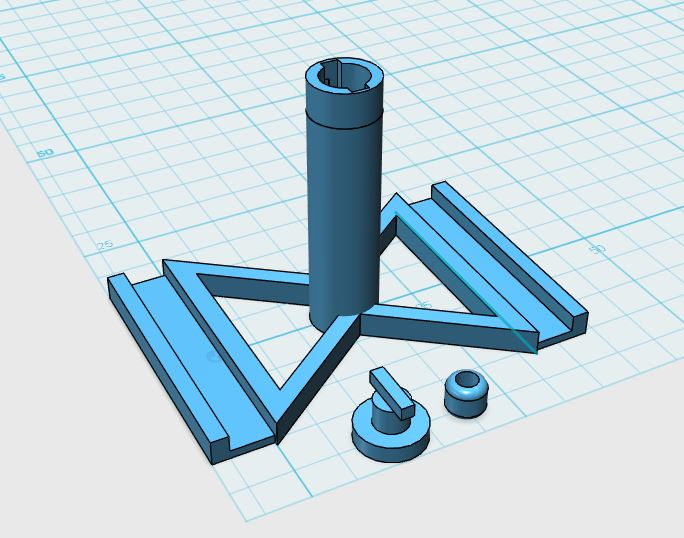
\includegraphics[width=0.4\linewidth]{images/PencilHolder.JPG}
	}\\
	\subfloat[Printed pencil holder\label{fig:pencilHolderReal}]{
		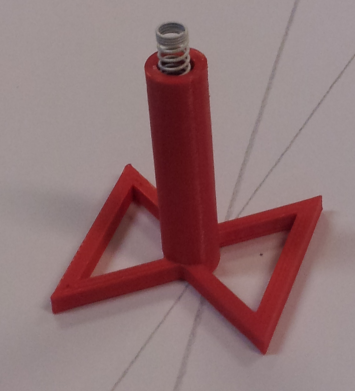
\includegraphics[width=0.4\linewidth]{images/penHolder.png}
	}
	\caption{3D printed utilities}
	\label{fig:3d}
\end{figure}
\begin{figure}[H]
	\centering
	\subfloat[Front of robot\label{fig:robotFront}]{
		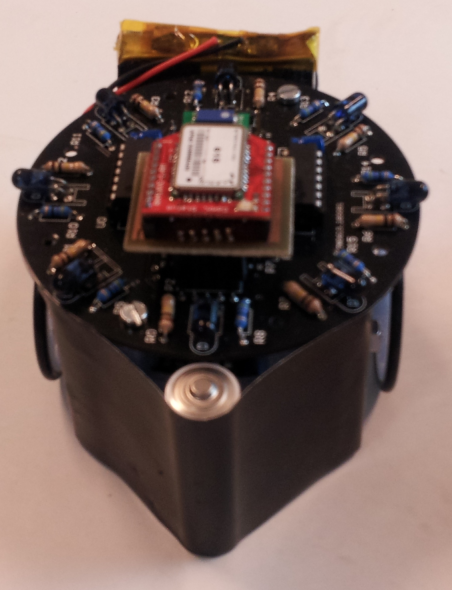
\includegraphics[width=0.4\linewidth]{images/robotFront.png}
	}
	\subfloat[Back of robot\label{fig:robotBack}]{
		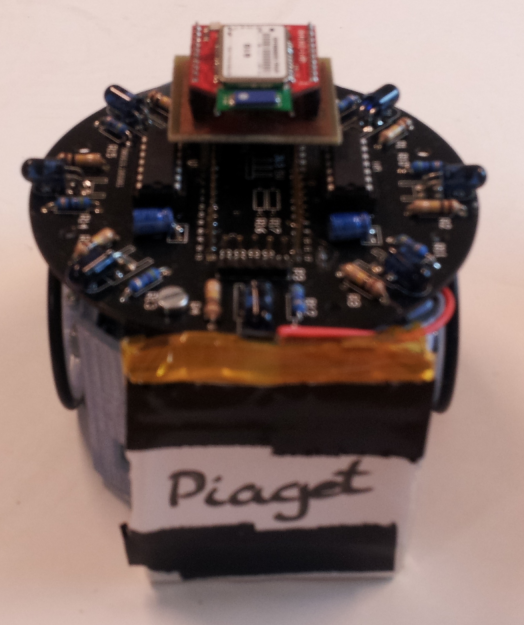
\includegraphics[width=0.4\linewidth]{images/robotBack.png}
	}\\
	\subfloat[Underside of robot\label{fig:robotUnder}]{
		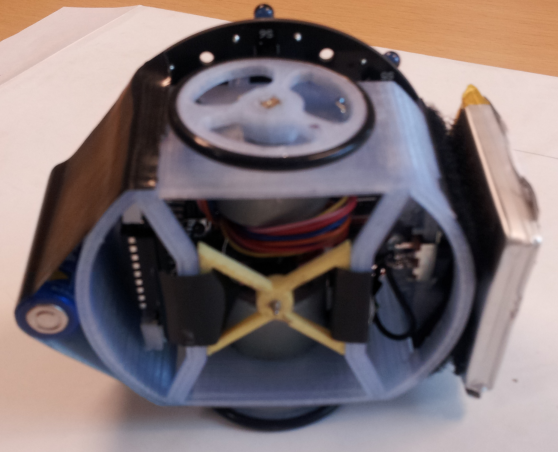
\includegraphics[width=0.4\linewidth]{images/robotUnder.png}
	}
	\subfloat[Robot drawing an angle\label{fig:robotDrawing}]{
		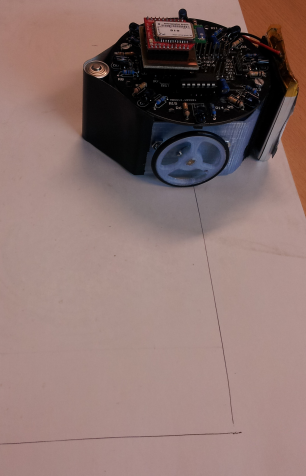
\includegraphics[width=0.4\linewidth]{images/robotDrawing.png}
	}
	\caption{Pictures of the robot}
	\label{fig:robot}
\end{figure}

\subsection{Bluetooth circuit board}
The \chirp team had previously tested using bluetooth communication between an android device and the robot. We therefore got help in creating the inital circuitry for our bluetooth module(figure~\ref{fig:circuitDrawing}). This drawing was at this point designed in the Eagle software in order to make it possible to produce at a later stage(~\ref{fig:circuitDesign}). 

\bigskip\noindent
It can be seen in figure~\ref{fig:circuitProto} that some soldering around the board was necessary in the prototype. The prototype did however lead us to believe that the circuit itself was functional and we were able to proceed with creating all the circuit boards that we needed. 
Figure~\ref{fig:circuitTrans} shows the template used in the etching process when creating these boards. While figure~\ref{fig:circuitboard} shows the circuit board alongside with the bluetooth module we used for our robots. The complete assembly of the robot can be seen in figure~\ref{fig:robotDrawing}.

\begin{figure}[!htb]
	\centering
	\subfloat[Inital circuit\label{fig:circuitDrawing}]{
		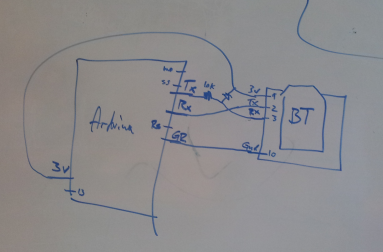
\includegraphics[width=0.4\linewidth]{images/bluetoothCircuit.png}
	}
	\subfloat[Created in circuit designer\label{fig:circuitDesign}]{
		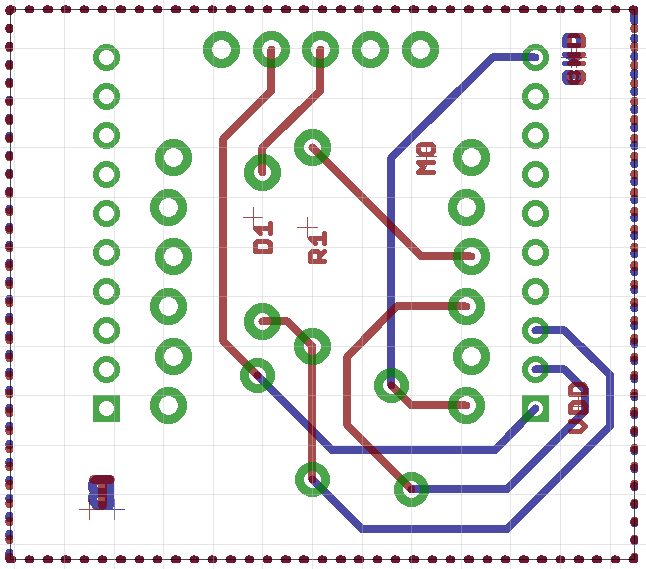
\includegraphics[width=0.4\linewidth]{images/circuitDrawing.PNG}
	}\\
	\subfloat[Prototype template\label{fig:circuitProtoTrans}]{
		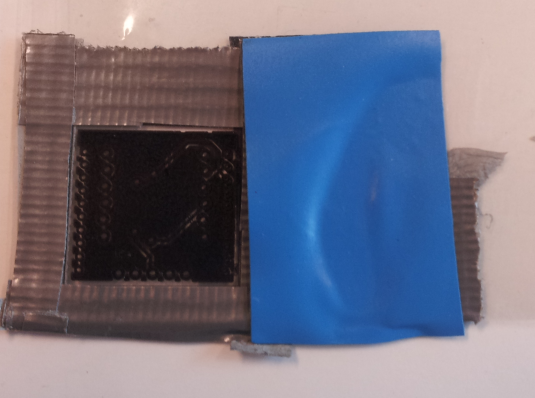
\includegraphics[width=0.4\linewidth]{images/bluetoothProtoTrans.png}
	}
	\subfloat[Prototype circuitboard\label{fig:circuitProto}]{
		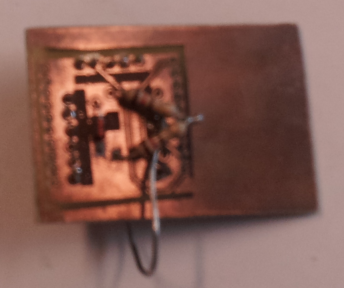
\includegraphics[width=0.4\linewidth]{images/bluetoothProto.png}
	}\\
	\subfloat[Finished template\label{fig:circuitTrans}]{
		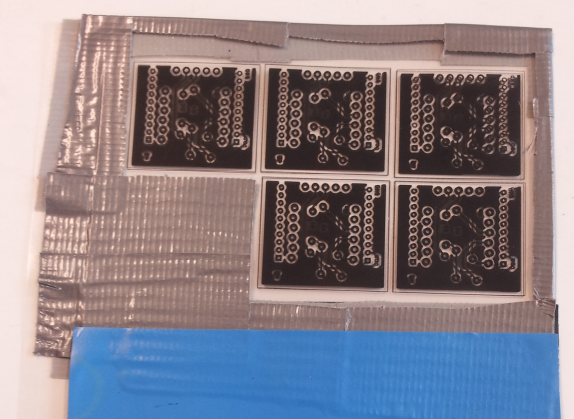
\includegraphics[width=0.4\linewidth]{images/bluetoothTrans.png}
	}
	\subfloat[Finished circuitboard\label{fig:circuitboard}]{
		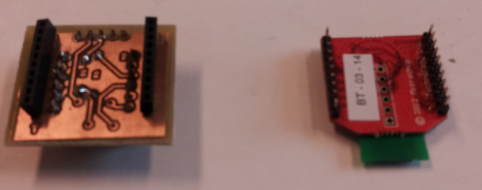
\includegraphics[width=0.4\linewidth]{images/bluetooth.png}
	}
	\caption{Circuit boards}
	\label{fig:circuit}
\end{figure}
